\documentclass[conference]{IEEEtran}

\usepackage{cite}
\usepackage{pslatex} % -- times instead of computer modern, especially for the plain article class
\usepackage[colorlinks=false,bookmarks=false]{hyperref}
\usepackage{booktabs}
\usepackage{graphicx}
\usepackage{xcolor}
\usepackage{multirow}
\usepackage{comment}
\usepackage{listings}
%\usepackage{flushend} % even out the last page, but use only at the end when there is a bibliography
\usepackage{listings}	% For inserting code
\usepackage{minted}		% For inserting code
\setminted[systemverilog]{
	tabsize=3
}
\setminted[C]{
	tabsize=3,
	breaklines
}
\setminted[scala]{
	tabsize=3,
	breaklines
}
\usepackage{xspace}		% For using \SV with trailing spaces
\usepackage{cleveref}	% Needed for correctly referencing listings

\newcommand{\code}[1]{{\small{\texttt{#1}}}}
\newcommand{\SV}{SystemVerilog\xspace}


% fatter TT font
\renewcommand*\ttdefault{txtt}
% another TT, suggested by Alex
% \usepackage{inconsolata}
% \usepackage[T1]{fontenc} % needed as well?

\usepackage{listings}

%\newcommand{\todo}[1]{{\emph{TODO: #1}}}
\newcommand{\todo}[1]{{\color{olive} TODO: #1}}
\newcommand{\martin}[1]{{\color{blue} Martin: #1}}
\newcommand{\simon}[1]{{\color{green} Simon: #1}}
\newcommand{\abcdef}[1]{{\color{red} Author2: #1}}
\newcommand{\rewrite}[1]{{\color{red} rewrite: #1}}
\newcommand{\ducky}[1]{{\color{orange} Richard: #1}}
\newcommand{\kasper}[1]{{\color{purple} Kasper: #1}}

% uncomment following for final submission
\renewcommand{\todo}[1]{}
\renewcommand{\martin}[1]{}
\renewcommand{\simon}[1]{}
\renewcommand{\kasper}[1]{}
\renewcommand{\ducky}[1]{}


\title{An Open-Source Verification Method with
Chisel and Scala}


%%% ZF
\usepackage{listings}
\lstset{
	columns=fullflexible,
	%        basicstyle=\ttfamily\footnotesize,
	basicstyle=\ttfamily\small,      
	%columns=fullflexible, keepspaces=true,
	numbers=left,    
	numberblanklines=false,
	captionpos=b,
	%	breaklines=true,
	escapeinside={@}{@},
	numbersep=5pt,
	language=C,
	tabsize=2,
	breakatwhitespace=true,
	breaklines=true,
	deletekeywords={for},
	%        keywordstyle=\ttfamily
	numbersep=5pt,
	xleftmargin=.10in,
	%xrightmargin=.25in
}



\begin{document}

\maketitle \thispagestyle{empty}


\begin{abstract}
Performance increase with general-purpose processors has come to a halt.
We can no longer depend on Moore's Law to increase computing performance.
The only way to achieve higher performance or lower energy consumption
is by building domain-specific hardware accelerators.
To efficiently design and verify those domain-specific accelerators, we need
agile hardware development.

This paper presents a combination of open-source tools for verifying
circuits described in mixed languages. It builds on top of the Chisel
hardware construction language and uses Scala to drive the verification. 
We also explore the testing strategy used in the Universal Verification Methodology
(UVM) in the context of verifying hardware described in Chisel.
\end{abstract}

\begin{IEEEkeywords}
digital design, verification, object-oriented programming
\end{IEEEkeywords}

\section{Introduction and Objectives}
\label{sec:objectives}

We can no longer depend on Moore's Law to increase computing performance~\cite{dark-silicon:2011}.
Performance increase with general-purpose processors has come to a halt.
The only way to achieve higher performance or lower energy consumption
is by building domain-specific hardware accelerators~\cite{domain-hw-acc:2020}.
These accelerators can be built in chips or in FPGAs in the cloud.
The production of a chip is costly. Therefore, it is essential to get
the design right at the first tape-out. Thorough testing and verification of the design is mandatory.

To efficiently develop and verify those accelerators, we can learn from software development trends such as agile software development~\cite{agile:manifesto}.
We believe that {\bf we need to adapt to agile hardware development}~\cite{henn-patt:turing:2019}.

Furthermore, as accelerators become part of the cloud service, i.e., FPGAs in the cloud,
software developers will increasingly need to adapt critical algorithms to FPGAs to enhance performance.
Hence, it is imperative to make accelerator design accessible for software developers.
By adapting hardware accelerator design to the methods and tools of contemporary software design,
it is possible to bridge both domains catering for a more uniform hardware/software development process.

Until a few years, the two main design languages Verilog and VHDL dominated the
design and testing of digital circuits.
%However, both languages are decades behind
%modern languages for software development.
However, compared to software development and testing, digital design and testing methods
and tools lack several decades of development. Within this project, we plan to
{\bf leverage software development and testing methods for digital design.}
This project explores the hardware construction language Chisel~\cite{chisel:dac2012} with Scala
and the Universal Verification Method (UVM) with SystemVerilog~\cite{SystemVerilog} for
the design and test of digital systems.

This project aims to develop a method and concrete tools for agile hardware development.
We will use tools, languages, development, and testing methods from the last decades in
software development and apply them to hardware design.
We aim to {\bf raise the tooling level for a digital design to increase productivity}.
Time for verifying (testing) of digital systems is about double the time of developing
them in the first place.
Therefore, this project's central focus is on {\bf applying software
testing methods for hardware testing}.

We will build a combination of open-source tools for verifying
circuits described in mixed languages (VHDL, SystemVerilog, and Chisel).
It builds on top of the Chisel hardware construction language and uses Scala to drive the verification. 
We will explore the testing strategy used in UVM in the context of verifying hardware described in Chisel.

This project proposes a research project that aims at building a testing framework
in Scala that takes the best methods from UVM and from decades of experience
in software testing.
The developed framework shall support mixed languages (VHDL, SystemVerilog, and Chisel)
to be able to integrate legacy code.
Furthermore, our aim is to build on open-source projects. Therefore, our
work will be in open-source as well.

\begin{itemize}
\item Maybe more ideas: \url{https://www.youtube.com/watch?v=dbOi_Gboi_0}, \url{https://www.youtube.com/watch?v=4FCZLrauDcE}
\item Higher-Order Hardware Design, meta-programming language and the actual hardware construction language are the same, usually Python or Perl scripts with strings
\item Have a measurable objective (LoC UVM vs Scala, SystemVerilog vs Chisel)
\item Chisel has all the Scala/Java tooling and libraries available, SystemVerilog is a niche language
\item Rise level of tooling, not necessarily level of abstraction in HW description
\item IDE
\item Namespace with packets make it easier to combine IPs
\item Industry issue is verification: how from Chisel to VHDL/Verilog
\item How much ASIC design is done in DK? Revenue numbers?
\item There are not enough HW designers and verification engineers available, so they shall be more productive
\end{itemize}

\section{Background and State-of-the-Art}
\label{sec:background}


\begin{itemize}
\item Verification (check what is current praxis)
\item cocotb
\item See pull request for ref to constraint random generation
\item Related work \url{http://koo.corpus.cam.ac.uk/drafts/tndjg-008-transactional-modelling-in-chisel.html}
\item SV OOP is not available for synthesize, functional coverage, another test case could be my S4NOC, reference models are usually written in SystemC to avoid licenses cost for the SW developer
\end{itemize}

\paragraph{Digital Design.}
VHDL and Verilog are the classic hardware description languages, first appeared in the 1980s.
SystemVerilog~\cite{SystemVerilog}, as an extension to Verilog, adds features from VHDL
for the hardware description and object-oriented features for verification.
Recent advances with SystemVerilog and Chisel \cite{chisel:dac2012, chisel:book} have
brought object-oriented programming into the digital design and verification process.

Chisel is a ``Hardware Construction Language'' embedded in Scala, to describe digital circuits~\cite{chisel:dac2012}.
Scala/Chisel brings object-oriented and functional programming into the world of digital design.
For hardware generation and testing, the full Scala language and Scala and Java libraries are available.
As Scala and Java's full power is available to the verification engineer,
the verification process is also made more efficient.


Chisel is a hardware construction language embedded in Scala.
Chisel allows the user to write hardware generators in Scala, an object-oriented and functional language.
For example, we read in the string based schedules for a network-on-chip
%\footnote{available at: \url{https://github.com/t-crest/s4noc/tree/master/noc/vhdl/generated}}
and convert them with a few lines of Scala code into a hardware table to
drive the multiplexer of the router and the network interface.

Chisel is solely a hardware \emph{construction} language, and thus all valid Chisel code
maps to synthesizable hardware.
By separating the hardware construction and hardware verification languages,
it becomes impossible to write non-synthesizable hardware and in turn, speeds up the design process.



On open source collection of SystemVerilog classes build the Universal Verification Method,
which is becoming popular in industry.
SystemVerilog has become a complex language with more than 250 keywords, and it is unclear
which tools support which language constructs for hardware description.
In contrast with Chisel, when the program compiles, it is synthesizable hardware.
Chisel is a small language, where the cheat sheet fits on two pages.
The power of Chisel comes from the embedding in Scala.
Furthermore, as classic hardware description languages are niche products, not
many tools or libraries are available. 
With Chisel on Scala we have the choice of different integrated development environments (IDE),
testing infrastructure (e.g., ScalaTest), and many free libraries.



Chisel and Scala are executing on the Java virtual machine and therefore have a very good
interoperability with Java. Therefore, we can leverage a large pool of Java libraries for
hardware design and  verification.
Furthermore, the name space of packets in Scala/Java simplifies integration of
external components.
Open source hardware components in Chisel can be organized like software
libraries at Maven servers.






%%%ZF
\paragraph{Testing Methods.}
Testing is crucial for making software and hardware reliable. The higher
expectation of software quality and shrinking development cycle have
driven programming language researchers and software engineers to
develop a spectrum of \emph{automated testing} techniques.
For example, continuous integration~\cite{duvall2007continuous} 
implements an agile method that automatically runs manually written
%State-of-the-art research in software engineering
%and programming languages address the following two challenges to
%achieve full test automation.

SystemVerilog adds object-oriented concepts for the non-synthesizable verification code.
The SystemVerilog direct programming interface~\cite{Doulos:SV:dpi} allows the programmer to call
C functions inside a SystemVerilog (UVM) testbench.
This enables co-simulation with a ``golden model'' written in C, and the
testbench verifying the device under test (DUT).
With ChiselTest we can co-simulate with Java and Scala models and use the Java Native Interface
to co-simulate with models in C.

The Java JNI (Java Native Interface) allows for a similar functionality in Java programs,
allowing them to call C functions and use their functionality.
By using Scala, which is built on Java, it is our hope to use the JNI together with Scala's test frameworks.
The aim is to develop a framework for co-simulation with Scala/Chisel testers and a
C-based golden model. This should allow companies to keep their existing C models,
but move their simulation workflow into Scala/Chisel testers.

The digital design described in Chisel can be tested and verified with
ChiselTest~\cite{chisel:tester2}, a non-synthesizable testing framework for Chisel.
ChiselTest emphasizes usability and simplicity while providing ways to scale up complexity.
Fundamentally, ChiselTest is a Scala library that provides access into the simulator through
operations like poke (write value into circuit), peek (read value from circuit, into the test framework), and step (advance time).
As such, tests written in ChiselTest are just Scala programs, imperative code that runs one line after the next.
This structure uses the latest programming language developments that have been implemented into Scala
and provides a clean and concise interface, unlike approaches that attempt to reinvent the wheel like UVM.

Furthermore, ChiselTest tries to enable testing best practices from software engineering.
Its lightweight syntax encourages writing targeted unit tests by making small tests easy.
A clear and clean test code also enables the test-as-documentation pattern,
demonstrating a module's behavior from a temporal perspective.

\paragraph{Determining Specification.}
The first challenge is how to determine the expected code outcome, or
called \emph{specification}.  Software developers often document
specifications within the software itself.  \emph{Property-based testing}
provides a convenient way of formulating specification as constraints
expressed in a domain-specific
language~\cite{DBLP:conf/icfp/ClaessenH00}.  For example, developers
in the Scala language can specify ``$n^2>0$ for all integer $n$'' in the
property-based testing library ScalaCheck~\cite{nilsson2014scalacheck}
as follows:
\begin{lstlisting}[numbers=none]
val propSquare = forAll {(n: Int) => n * n > 0}
\end{lstlisting}
An efficient approach to obtaining such specifications is to learn from
historical bug patterns. Such patterns are gathered in pattern-based
software analysis tools, e.g., in
FindBug~\cite{DBLP:conf/paste/AyewahPMPZ07} or
Scalafix~\cite{web:scalafix}.  Recently, a specification for robotic
software is obtained by studying bugs fixed on the Robot
Operating System~\cite{nielsenFSW2020dependencybugs}.





%% ZF. This is commeented out because we have decided to not write on
%% the WP related to sanitizers.

%% Another way to generate specification is to use \emph{sanitizers}
%% in compilers. Sanitizers are a common compiler feature that
%% automatically injects run-time checks to capture certain failure
%% conditions~\cite{DBLP:conf/usenix/SerebryanyBPV12}. For example,
%% Google's undefined behavior sanitizer UBSAN checks whether a
%% floating-point variable equals 0 before a division by it; Google's
%% address sanitizer ASAN targets illegal memory access. While
%% sanitizers do not deal with functional correctness as unit tests
%% do, they check low-level, sometimes security-related properties,
%% such as use-after-free, array-index-out-of-bound, or race
%% conditions.

\paragraph{Generating Test Inputs.}
The second challenge is how to generate interesting test inputs.  The
state-of-the-practice uses \emph{fuzzing}, which has emerged as one of
the most effective testing techniques for discovering reliability
issues in software~\cite{takanen2018fuzzing}.  Google's OSS-Fuzz
project, for example, has filed over 20 000 bugs in 300 open-source
projects (as of June 2020)~\cite{web:oss-fuzz}.  Fuzzing techniques
generate random inputs and improve them based on observed code status,
e.g., crashes or code
coverage~\cite{DBLP:journals/tse/BohmePR19,DBLP:conf/pldi/FuS17}.
Property-based testing~\cite{DBLP:conf/icfp/ClaessenH00}, which is
initially designed for testing functional programming languages, uses
random data generation, a form of plain fuzzing. For example, by
invoking {\tt propSquare.check} with ScalaCheck (mentioned above), where {\tt
  propSquare} is the constraint $n^2>0$ for all integers $n$, we can
immediately get an input $n$ that falsifies the constraint:

\begin{lstlisting}[numbers=none]
scala> propSquare.check
       ! Falsified after 1 passed tests.
      > ARG_0: 0
      > ARG_0_ORIGINAL: 1083860448
\end{lstlisting}
 ScalaCheck first finds that n = 1083860448 produces an overflow
 wrapped to a negative (thus $n^2>0$ fails). The input is then
 ``shrunk'', in the terminology of property-based testing, to a smaller
 one, namely 0 in this case.



\section{Coverage in Chisel}
One of the main tools used in verification is Test Coverage. This allows verification engineers to measure their progress throughout the testing process and have an idea of how effective their tests actually are. Coverage can be separated into two distinct categories: Code coverage and Functional coverage. Code Coverage defines a quantitative measure of the testing progress, \textit{"How many lines of code have been tested?"}, whereas Functional Coverage gives a rather qualitative measure, \textit{"How many functionalities have we tested?"}.  Our solution would give the verification engineer access to two ways of obtaining their code coverage and new constructs allowing the definition of a verification plan and the creation of a functional coverage report directly integrated into the Chisel testing framework.\\

\paragraph{Code Coverage with Treadle}  
The first part of our solution is about code coverage, more specifically line coverage that was added to the Treadle FIRRTL execution engine. Treadle is a common FIRRTL execution engine used to simulate designs implemented in Chisel. This engine runs on the FIRRTL intermediate representation code generated by a given Chisel implementation and allows one to run user-defined tests on the design using frameworks like \textit{Chisel Testers2} or the more standard \textit{iotesters}. In our pursuit of creating a verification framework, we found that one way to obtain line coverage would be to have our framework run on an extended version of Treadle that was capable of keeping track of said information.\\\\
The solution that was used to implement line coverage was based off of a method presented by Ira. D. Baxter~\cite{branch-cov-made-easy:2002}. The idea is to modify the DUT's source code, before generating the \textit{AST} (Abstract Syntax Tree) used to execute the tests, by adding additional outputs for each multiplexer in the design. These new ports, which we will call \textit{Coverage Validators}, are set depending on the paths taken by each multiplexer and that information is then gathered at the end of each test and maintained throughout a test suite. Once the testing is done, we used the outputs gathered from the \textit{Coverage Validators} to check wether or not a certain multiplexer path was taken during the test, all of this resulting in a branch coverage percentage. Finally a \textit{Coverage Report} is generated containing the following: 
\begin{itemize}
\item The multiplexer path coverage percentage.
\item A modified version of the FIRRTL code of the DUT containing prefixes for each line telling us whether it was covered by a test or not.
\end{itemize}
\begin{verbatim}
COVERAGE: 50.0% of multiplexer paths tested
COVERAGE REPORT:

+ circuit Test_1 :
+   module Test_1 :
+     input in$a : UInt<1>
+     input in$b$0 : UInt<2>
+     input in$b$1 : UInt<2>
+     input clock : Clock
+     output io_cov_valid_0 : UInt<1>
+     output io_cov_valid_1 : UInt<1>
+     output out : UInt<2>
+   
+     io_cov_valid_0 <= in$a
-     io_cov_valid_1 <= not(in$a)
+     out <= mux(in$a, in$b$0, in$b$1)
\end{verbatim}
The example above is taken for a simple test, where we are only testing the path where \texttt{in\_a} is 1. This means that, since we only have a single multiplexer, only half of our branches have been tested and we would thus want to add a test for the case where \texttt{in\_a} is 0. The report can thus be interpreted as follows:  
\begin{itemize}
\item "\texttt{+}" before a line, means that it was executed in at least one of the tests in the test suite.
\item "\texttt{-}" before a line, means that it wasn't executed in any of the tests in the test suite.\\
\end{itemize}

Treadle thus allows us to obtain coverage at the FIRRTL level. A more interesting result would be if the FIRRTL line coverage would be mapped to the original Chisel source. This is possible but challenging, since Treadle only has access to the original source code through \textit{Source locators} which map some of the FIRRTL lines back to Chisel. This means that the code can only be partially mapped and the remainder will have to be reconstructed using some smart guessing.\\

\paragraph{Functional Coverage directly in Scala}
Functional Coverage is on the principal tools used during the verification process, since it allows one to have a measurement of \textit{"how much of the specification has been implemented correctly"}. A verification framework would thus not be complete without constructs allowing one to define a verification plan and retrieve a functional coverage report. The main language used for functional coverage is \textit{SystemVerilog}, which is why our solution is based on the same syntax. There are three main components to defining a verification plan: 
\begin{itemize}
\item \texttt{Bin}: Defines a range of values that should be tested for (i.e. what values can we expect to get from a given port).
\item \texttt{CoverPoint}: Defines a port that needs to be sampled in the coverage report. These are defined using a set of bins.
\item \texttt{CoverGroup}: Defines a set of \texttt{CoverPoint}s that need to be sampled at the same time.
\end{itemize}
Using the above elements, one can define what's known as a verification plan, which tells the coverage reporter what ports need to be sampled in order to generate a report.
In order to implement said elements in Scala we needed to be able to do the following:
\begin{itemize}
\item Define a verification plan (using constructs similar to \texttt{coverpoint} and \texttt{bins}).
\item Sample DUT ports (for example by hooking into the \textit{Chisel Testers2} framework).
\item Keep track of bins to sampled value matches (using a sort of DataBase).
\item Compile all of the results into a comprehensible Coverage Report.
\end{itemize}
Implementing these elements was done using a structure where we had a top-level element, known as our \texttt{Coverage Reporter} which allows the verification engineer to define a verification plan using the \texttt{register} method, which itself stores the \texttt{coverpoint} to \texttt{bin} mappings inside of our \texttt{CoverageDB}. Once the verification plan is defined, we can sample our ports using the \texttt{sample} method, which is done by hooking into \textit{Chisel Testers2} in order to use its peeking capabilities. At the end of the test suite a functional coverage report can be generated using the \texttt{printReport} method, which shows us how many of the possible values, defined by our bin ranges, were obtained during the simulation.
\begin{lstlisting}[language=scala]
val cr = new CoverageReporter
cr.register(
    //Declare CoverPoints
    //CoverPoint 1
    CoverPoint(dut.io.accu , "accu",
        Bins("lo10", 0 to 10)::
        Bins("First100", 0 to 100)
        ::Nil)::
    //CoverPoint 2
    CoverPoint(dut.io.test, "test", 
        Bins("testLo10", 0 to 10)
        ::Nil)::
    Nil,
    //Declare cross points
    Cross("accuAndTest", "accu", "test",
        CrossBin("both1", 1 to 1, 1 to 1)
        ::Nil)::
    Nil)
\end{lstlisting}
The above code snippet is an example of how to define a verification plan using our coverage framework. The concepts are directly taken from \texttt{SystemVerilog}, so it should be accessible to anyone coming from there. One concept, that is used in the example verification plan, which we haven't presented yet is the idea of \textit{Cross Coverage} defined using the \texttt{Cross} construct. \textit{Cross Coverage} allows one to specify coverage relations between CoverPoints. This means that a cross defined between, let's say, \texttt{coverpoint a} and \texttt{coverpoint b} will be used to gather information about when \texttt{a} and \texttt{b} had certain values simultaneously. Thus in example verification plan we are checking that \texttt{accu} and \texttt{test} take the value 1 at the same time.\\
Once our verification plan is defined, we need to decide when we want to sample our cover points. This means that at some point in our test, we have to tell our \texttt{CoverageReporter} to sample the values of all of the points defined in our verification plan. This can be done, in our example, simply by calling \texttt{cr.sample()} when we are ready to sample our points. Finally once our tests are done, we can ask for a coverage report by calling \texttt{cr.printReport()} which results in the following coverage report: 
\begin{verbatim}
============== COVERAGE REPORT ==============
================ GROUP ID: 1 ================
COVER_POINT PORT NAME: accu
BIN lo10 COVERING Range 0 to 10 HAS 8 HIT(S)
BIN First100 COVERING Range 0 to 100 HAS 9 HIT(S)
============================================
COVER_POINT PORT NAME: test
BIN testLo10 COVERING Range 0 to 10 HAS 8 HIT(S)
============================================
CROSS_POINT accuAndTest FOR POINTS accu AND test
BIN both1 COVERING Range 1 to 1 CROSS Range 1 to 1 
HAS 1 HIT(S)
============================================
\end{verbatim}

\section{Research Plan}


%%%ZF
%\subsection{WP1}
As prerequisites, all researchers involved in this project will need to learn
languages and tools involved in the project and related work.
They will learn about the Scala programming language and ScalaCheck
(a Scala implementation of the property-based testing) on the software side.
On the hardware side,
the researchers need to get familiar with Chisel, SystemVerilog, and
UVM.


\paragraph{Hardware Generators.}

The productivity of hardware design can be greatly increased by developing so-called
hardware generators. A hardware generator is a program that can generate a configurable
hardware description.
Scala with functional programming is an excellent basis for developing a methodology for the
development of such hardware generators.


%\subsection{WP2}
\paragraph{Property-based Testing.}
As a starting point, we will use ScalaCheck, an implementation of
property-based testing in Scala, for hardware testing. We will invite
hardware developers to write properties as constraints (like
propSquare above), and then we will use ScalaCheck to validate or
refute those constraints. Property-based testing has seen notable
successes previously, such as in locating a long-standing concurrency
bug in the Erlang database server~\cite{DBLP:conf/erlang/HughesB11};
it was also used by Ericsson to test its media
proxy~\cite{DBLP:conf/erlang/ArtsHJW06}, by Volvo to test car
communications protocols~\cite{DBLP:conf/icst/ArtsHNS15}.


\paragraph{Co-simulation.}

\todo{A figure would be nice.}

\begin{itemize}
\item One use case for evaluation: cosimulation of a RISC-V simulator (Tommy) with an OS RISC-V HW 
\item Ptolemy~\cite{ptolemyII-book} can be used to co-simulate the environment, supporting a model based design.
\item Integration of C/C++ based models in the verification with Scala
\item Java/Scala in UVM
\item Hw/sw co-verification with Scala and so on, e.g., run an application on a SW processor model exploring some hardware artifacts (could be S4NOC)
\item Model based design (Jan) with co-simulation
\end{itemize}

\paragraph{Assertions.}

\begin{itemize}
\item assertions during simulation
\item Assertion ave been long part in SW, begin of C, but seldom used in HW and more complex assertions are interesting, such as when req is asserted, an ack has to become active within 5 clock cycles
\end{itemize}

\paragraph{Constraint Random Testing and Fuzzing Techniques.}

Constraint random testing in hardware is similar to fuzzing in software testing.
We will add support for constrain random testing to ChiselTest~\cite{chisel:tester2}.
Once we have tools to instrument the hardware under test with a user-written
specification or automatically generated specification, we will be able to use fuzzing techniques
to validate those specifications. To this end, we will work
with our industrial collaborators to get access use cases serving
as the DUT.

\paragraph{Test Coverage.}
Tests of the hardware model are traditionally done by ``directly'' validating the features listed in the specifications. As shown in \cite{spear2008systemverilog}, this methodology increases linearly with the complexity of the design. Opposite to direct testing, is random testing. Random testing focus on validating the design on a purely random set of inputs which may or may not detect all the corner cases \cite{mehta2017a}. An alternative approach is to constrain the randomization of input of the test to reduce the design validation time. By combining test coverage (pargraph \ref{test-coverage}) and constrained random stimuli, it is possible to narrow down the corner cases by focusing the test on areas where coverage is lacking. Currently, Hardware verification languages such as SystemC, System Verilog and ``e'' integrate a special syntax to enable this validation technique. However, given their relative old design, such features are hard to extend \cite{haedicke2012crave} \cite{le2015boosting}. On the contrary, new programming languages like Python and Chisel provide a more extensible syntax and builtin package managers that easily allows the integration and extension of a similar feature in the language. Random constraints are modelled base on top of an ``Random'' data type objects that contain random variables and user-defined constraints.  The combination of the constraints applied to a ``Random'' object determines the possible values that can be assigned to the random variables. This approach allows the user to build generic reusable objects that can be later extended or constrained based on the specifications \cite{cieplucha2016new}\cite{mehta2017a}. As for now, solution like cocotb \cite{rosser2018cocotb}\cite{cocotb2020Sep} have already extensions library that combine Constraint Random Verification and Test Coverage \cite{mciepluc2020Sep}. In the cocotb implementation, the constraint random verification module leverage the general-purpose library python-constraint \cite{python-constraint2020Sep} to solve constrained constraint satisfaction problem (CSP) and create the ``Random'' objects. A similar result can also be achieved in Chisel by combining general-purpose constraint problem solver libraries like \cite{chocoteam2020Sep} or \cite{BibEntry2020Sep}.

Code coverage is a useful tool for verifying digital designs
since it allows one to see which parts of their design have actually been tested correctly. 
We will implement coverage inside of the execution engine of the Chisel simulator using a technique
presented by Ira. D. Baxter~\cite{branch-cov-made-easy:2002}.
We will add a method to specify \textit{functional coverage points}, also known as
\textit{coverage groups} in SystemVerilog.


Treadle, which is a simulation engine for Chisel, does not contain support for measuring code coverage.
We will added branch coverage to Treadle so that one can see which lines of
LoFIRRTL code, the intermediate representation used inside of Treadle, were covered by a series of tests
and then know, using that information, which multiplexer paths were tested. 
Furthermore, we plan to map the results obtained with LoFIRRTL code back to the source Chisel description.
This mapping can be done using treadle's internal ``source trackers'' that associate some FIRRTL lines back
to their chisel source. Once that is done, it will be interesting to move from branch coverage to functional
coverage, which would require a way to define \textit{functional coverage points} also known as
\textit{coverage groups} in SystemVerilog.

\begin{itemize}
\item On coverage and cover points in proposal (coverage of the RTL hardware, but also on the generator (Jack's comment, see \url{https://gitter.im/freechipsproject/chisel3?at=5f63c878603d0b37f43b67f3})
\item Also have range coverage on individual signals and the matrix of 2 or more (see UVM example).
\end{itemize}



\paragraph{Verification Framework.}

We will develop an object-oriented and functional framework for verification in Scala.
This framework is inspired by UVM, but will leverage Scala's conciseness with the
combination of object-oriented programming with functional programming.
An initial experiment of testing the accumulator circuit of the Leros processor~\cite{leros:arcs2019}
showed the that a test written with UVM was about 800 lines of code, where a Scala based
test was around 80 lines of code~\cite{verify:chisel:2020}.
However, UVM supports more functionality that a plain ChiselTest in Scala.

Within our verification framework, we will support mixed language verification.
Verilog can easily be combined with Chisel, as Chisel generates Verilog, and
we will use ChiselTest as a driver for the open-source Verilog simulator Verlator.
With Yosys synthesis suite~\cite{Yosys} and GHDL~\cite{ghdl}
we will translate VHDL into Verilog.

A verification method is only usable when it can handle mixed-source designs.
This means a Scala driven method must be able to test components written in Verilog,
VHDL, and SystemVerilog.

Chisel has support for black boxes, which allows the use of Verilog code within the Chisel design.
Therefore, it is relatively easy to integrate Verilog components when wrapped into a black box.
However, this forces Chisel to use Verilator instead of Treadle to run the simulation, impacting
startup time.

Chisel does not fully support VHDL. It can support VHDL using VCS, but there is no
open-source solution available for VHDL simulation. For companies with a lot of source code written in VHDL this is a concern, as they must be able to integrate their existing IP in a Scala/Chisel based design and verification workflow.
All major commercial simulation and synthesis tools support mixed-language designs, but no open-source tools exist that provide the same functionality.

To alleviate this issue, the open-source Yosys synthesis suite \cite{Yosys} can be used. Yosys is an open-source digital hardware synthesis suite for Verilog. Yosys also has a variety of plugins, one of these being a plugin for using GHDL \cite{ghdl}, an open-source VHDL simulator. By using Yosys in conjunction with GHDL, VHDL files are compiled to an RTL-based intermediate representation, which is then written to a Verilog file using Yosys. GHDL has full support for IEEE 1076 VHDL 1987, 1993, 2002, and a subset of 2008. The workflow can be seen in Figure \ref{fig:VHDL2Verilog}. A working solution named VHDL2Verilog has been made for this, which has been tested with certain simple VHDL designs \cite{vhdl2verilog}.



\begin{itemize}
\item Bus functional models
\item Multiple languages
\item Still talk about a small example taking it through all variations
\item WP on VHDL generation from Chisel for better verification
\item p69: HDL models are SW projects
\end{itemize}



%% Let us consider this one below as a bonus WP in our backyard.
%% \subsection{WP2} 
%% We can then consider to generate specification automatically, \`a la
%% sanitizers used in the compiler techniques. This WP focuses on
%% low-level properties derived from the program syntax, {\em, e.g.},
%% accessing an array should be within a bound, or performing an
%% arithmetic calculation should not overflow.



%% \paragraph{MS2.} The milestone in this WP is to develop a program transformer
%% that injects in the software source, or its binary form, a list of
%% low-level specifications.

%% Related to this WP, our project collaborator Zhoulai Fu (together with
%% a hired security hacker) used sanitizers to find more than 200 bugs in
%% the Robot Operating System
%% (ROS)~\cite{web:ros-sanitizer-logs}. Besides, Zhoulai Fu has developed
%% several program transformers previously for testing floating-point
%% computation~\cite{DBLP:conf/pldi/FuS19,DBLP:conf/oopsla/FuBS15}.



\paragraph{Learning Specification from Historical Bug Patterns.}
We will consider generating specifications from previously known bug
patterns.  We will collaborate with our hardware engineers to explore
a history of hardware issues triggered by software defects and get
patterns from which we generate specification.  Such bug patterns in
Java, for example, can be found in \cite{web:findbugs_bugs}.  This
step will generate specification in a syntax-driven way, relating to
the expected functional behavior of the hardware.



%% Related to this, our collaborator Zhoulai Fu has worked on a
%% comprehensive study of developing bug finders by learning from history
%% bug patterns in the Robot Operating
%% System~\cite{nielsenFSW2020dependencybugs} 


%% Let us consider this as another backyard WP.
%% \subsection{WP5} We plan to deploy our automated testing solution  in a continuous
%% integration service, presumably on the cloud, such as Jenkins or
%% Travis~\cite{DBLP:journals/tse/GallabaM20}. For each code commit, the
%% service will automatically generate the specification as implemented
%% in WP2 and WP3, and then will generate test data with a fuzzing engine
%% as in WP4.

%% \paragraph{MS5.} The milestone is to have the server established that implements
%% the workflow. It should produce a detailed status report for each
%% commit.  A similar kind of status report can be found in Google's
%% OSS-Fuzz (Continuous Fuzzing for Open Source
%% Software)~\cite{web:oss-fuzz} for example.


\paragraph*{Dissemination and Publication}

Scientific results will be published and presented at international
conferences (e.g., DATE, DAC, CAV, FPL, ISCAS, FPGA) and in relevant scientific journals
and two PhD theses.
%We expect that most tasks will result in at least one publication.
%One PhD theses will publish the results from the project.
We aim to publish in open access, to a large extent, in the gold open access model.
However, publishers such as ACM also allow publishing in green open access
at no additional cost, where a pre-print version of a paper can be uploaded,
for example, to ArXiv.

The results from the project will be available as open-source under the
industry-friendly BSD license.
Open-source research projects attract
other researchers, developers, and industrial partners
to use and build on the results of the project.
A project web site will host the project documentation, the published papers, and the design's source code.
We will provide unrestricted and cost-free digital access to all research and development results.

We will use the developed method and tools to train a new generation of HW/SW engineers
at DTU and ITU.
In the middle of the project, we will have a coordination workshop with the project partners.
In the end, we will organize a design and verification workshop, including a hands-on tutorial,
open to all interested companies, and students from DTU and ITU.

\section{Practical Feasibility}

The Embedded Systems Engineering section at DTU Compute provides
the intellectual environment and the infrastructure (e.g., regression test server...) that we need for an ambitious research project.
Furthermore, DTU Compute provides the infrastructure (e.g., an automatic test
environment for regressions tests, web server).







\paragraph*{Use Cases}

We will have several non-trivial use cases from industry and from our own development to verify
our development.
Microchip provides the specification of a hardware sorting algorithm.
From WSA we will use a decimation filter written in VHDL.
From our research we will use a multicore device, a network-on-chip~\cite{s4noc:nocarc2019},
to explore concurrent, transaction based verification.

In the process of the research, the the specification of the hardware sorting algorithm provided by Microchip was 
successfully implemented in a parameterized priority queue module in chisel. The sorting is based on heap sort which allows for efficient 
sorting of the enqueued elements. Testing and verification of the component was conducted in scala with chiseltest. A reference model written in scala
was used to verify outputs after driving random inputs onto the component. In order to evaluate coverage of those
random test sequences, the developed coverage report functionality was successfully employed.



%\vspace{-5mm}
\paragraph*{Tasks, Milestones, and Timetable}





\bibliographystyle{abbrv}
%\bibliography{myown,jsp,noc,misc,msbib}
\bibliography{../msbib,testing,../chisel-uvm}


\section{Ideas, Questions, TODOs}



\begin{itemize}
\item Look at the TODO list in infinit project
\item DeepSpec or DeepSp?? end-to-end for Chisel
\end{itemize}


\subsection{TODO}

\section{UVM, SystemVerilog and verification}
The purpose of this document is to outline my (Kasper) findings during the course of the Chisel-UVM project. It should serve as a reference on what the UVM can do, how it works, and how some of this (namely the SystemVerilog Direct Programming Interface (DPI)) may be implemented in a Scala based testing framework.

\section{UVM}
The Universal Verification Methodology (UVM) is a verification framework built on top of the testing capabilities of SystemVerilog. Prior to the introduction of the UVM, the major EDA simulation vendors supported diferent frameworks / methodologies. This meant that a verification environment designed for one simulator might not run under another simulator. The main purpose of the UVM was to standardize the testing framework used across EDA vendors, making it easier for users to use their testbenches across different software suites.

%% The below is taken from our chisel-uvm paper
The testbench in the UVM is built up around a number of components.
Each component performs only one task in the testbench, allowing the engineer to make changes to some components without affecting others. 
For example, the sequencer is the component responsible for generating transactions for the DUT, whereas the driver is responsible for converting the transaction into pin-level wiggles, i.e., generating correct start/stop conditions and
driving signals. If a new sequence of transactions is to be generated, only the sequencer is affected. Likewise, the sequencer does not care how the transactions are converted into pin-level signals---this is the sole responsibility of the driver. This separation into several components results in a more structured testbench design as there are fewer dependencies than in a monolithic testbench.

The main components of a UVM testbench are as follows:

    A \textit{Sequence(r):} defines the order of transactions necessary for a given purpose, e.g., synchronization or reset sequence. The sequencer is responsible for transferring the transactions, defined by the sequence, to the driver.
    
    A \textit{Driver} converts transactions into pin-level signals and drives these signals onto the DUT.
    
    An \textit{Interface} is a SystemVerilog construct which allows the user to group related signals. A DUT may have several interfaces attached.
    The interface is used to avoid hooking directly into the DUT, making it easier to test multiple DUT versions.
    
    A \textit{Monitor} monitors all traffic on the interface, converting pin-level signals into transaction-level objects that can be operated on by other components, such as a coverage collector or scoreboard.
    
    An \textit{Agent} encapsulates monitor, sequencer and driver, setting configuration values. Agents may be set active or passive (with or without a driver and sequencer). An agent is useful when it is necessary to have multiple instances of the same components, e.g., when a 4-port network switch needs four identical drivers with different configurations.
    
    A \textit{Scoreboard} is used to check whether correct functionality is achieved. Usually does so by using a ``golden model'' for co-simulation via the SystemVerilog direct programming Interface.
    
    The \textit{Environment} is used to configure and instantiate all child components. Environments are typically application-specific and may be modified by the test.
    
    The \textit{Test} is the top-level verification component. The test designer may choose to perform factory overrides of classes and set configuration values here, which modify the child components.

As shown above, even a ``Hello, World'' example using the UVM requires that the user understands how and why each of the different UVM components should be used. The use of so many components causes UVM to have a very steep learning curve, which may discourage adoption. This also means that UVM is not the proper testing methodology for small designs or one-off tests due to the initial workload.
However, once the initial setup of the testbench is finished for large and complex designs, generating new tests becomes easier.

\subsection{Scoreboard and DPI}
The purpose of the scoreboard is to ensure that the DUT matches specification. When using directed tests (i.e. hand-written tests meant to test a single part of the specification), this may be as simple as constructing a list of input/output values and checking these in order. When using randomized testing, the scoreboard is usually implemented as a software model (sometimes called a golden model) which is defined to be correct. The software model should exactly mimic the functionality of the DUT, and thus provide the same outputs given the same inputs. 

The scoreboard may be implemented purely in SystemVerilog, or it may be implemented in a C-like language (C, C++ or SystemC). One of the benefits that \SV adds to the verification environment is the ability to interface with C-code through the use of the \SV Direct Programming Interface (DPI). This is an interface which allows C code to be called from inside the \SV testbench, and likewise allows for \SV code to be called from inside of a C program. Programming low-level simulations of hardware is most likely easier in C than in plain \SV. In listing \ref{lst:dpi} is shown a simple example of some SystemVerilog code calling C code through the \SV DPI. 

Notice the inclusion of the header file \texttt{svdpi.h}, which contains the definitions necessary for interoperability. Once this is done, the function must be imported in \SV by use of the \texttt{import "DPI-C"} statement, after which the function may be called as any other \SV function. Using the DPI is surprisingly simple and painless, and makes it very simple to integrate a C model in the testbench.

It should be noted that a scoreboard doesn't necessarily "rate"\, the performance of the DUT by comparing it to other modules, as one might expect from the name. The DUT is only compared against the reference model, and the "rating" is how many assertions pass/fail in a given test.

\begin{listing}[htbp]
\begin{minted}{C}
//hello.c
#include "svdpi.h"
#include <stdlib.h>

void c_hello(char* name) {
	printf("Hello from C, %s", name);
}
\end{minted}
\begin{minted}[breaklines]{systemverilog}

//hello.sv
module tb;
import "DPI-C" function void c_hello(string name);

	initial main();
	task main();
		c_hello("SystemVerilog");
	endtask
endmodule

// Outputs: "Hello from C, SystemVerilog"
\end{minted}
\caption{Short example showing how to use the \SV DPI to execute C-code from within \SV.}
\label{lst:dpi}
\end{listing}

\subsection{Constrained random verification}

Most UVM testbenches employ "Constrained Random Verification"\, (CRV) for generating test stimulus. This is as opposed to using directed testing, where input vectors are predefined to test a certain behaviour. With CRV, random test stimuli are generated. The "Constrained" part of CRV implies that these values aren't entirely random, but are chosen to fulfill a series of criteria. If eg. the DUT is an ALU with a 5-bit opcode field of which only 20 bit-patterns are used, it would be prudent to only generate the 20 valid opcodes for most test purposes. Specific tests could then be written to ensure proper operation if an invalid opcode was asserted.

An example of a class with randomized variables is seen in listing \ref{lst:crv}. 

The keyword \texttt{constraint} is used to constrain a variable defined with the \texttt{rand} keyword.
One randomized variable, \texttt{bcd}, is a 4-bit field which only takes on values in the range 0 and 9. 
The field \texttt{value} has a $1/3$ chance of being 0, $1/3$ of being 255 and $1/3$ of being any other value. 
The fields \texttt{a,b,c} must satisfy $0<a<b<c$. 
The field \texttt{op} has no constraints, and will thus randomly toggle between  0, 1, 2 and 3, the only values it can take on.

\begin{listing}[htbp]
\inputminted{systemverilog}{snippets/Myclass.svh}
\caption{Example SystemVerilog code showing how different values are constrained.}
\label{lst:crv}
\end{listing}

In listing \ref{lst:usingcrv}, an object of type \texttt{Myclass} is instantiated and randomized using the \texttt{mc.randomize()} command. Finally, the \SV function \texttt{\$display} is used to print the value of the BCD field. The \texttt{randomize} keyword is a \SV construct which will try to randomize all random fields of given class.

\begin{listing}[htbp]
\begin{minted}{systemverilog}
//top.sv
`include "Myclass.svh"
module top;
  Myclass mc;
  initial begin;
    mc = new;
    mc.randomize();
	 $display(mc.bcd);
  end
endmodule
//Outputs a random value in the range [0:9]
\end{minted}
\caption{Example SystemVerilog code showing how to instantiate and randomize a class with random fields.}
\label{lst:usingcrv}
\end{listing}

\subsection{Coverage collection}
The purpose of coverage collection, in this case functional coverage collection, is to check whether all "necessary"\, (as defined by the verification engineer) input combinations have been generated. For the ALU mentioned above, it might be interesting to check whether all opcodes work correctly when asserted after a reset, and whether over/underflow flags are correctly set when performing arithmetic operations. In general, functional coverage is concerned with evaluating whether all functionality of a device has been tested. This is opposed to line coverage, which evaluates which lines of code were run during a simulation.

\begin{listing}[htbp]
	\inputminted{systemverilog}{snippets/Cover.svh}
	\caption{Examle SystemVerilog code showing how covergrups and coverpoints are organized.}
	\label{lst:cov}
\end{listing}

An example of functional coverage collection is seen in listing \ref{lst:cov} where the randomized values from before are covered. A \textit{covergroup} is a label used to collect relevant values under the same heading. A \textit{coverpoint} is a directive instructing the simulator that the given value should be monitored for changes. In the declaration of the coverpoint, several \textit{bins} are generated. These bins correspond to the bins of a histogram. Every time an event occurs which matches the declaration inside a bin, the counter associated with that bin is incremented by one. An event may cause multiple bins to increment at the same time.



In the coverage declarations shown in listing \ref{lst:cov}, the covergroup \texttt{cg\_bcd} only covers one field, \texttt{bcd}. The bin is labeled by prepepending \texttt{BCD:} in front of the \textit{coverpoint} directive. 10 bins are generated which each sample the values 0-9, and the remaining values 10-15 are sampled into the default bin \texttt{others}. 

In the covergroup \texttt{cg\_others} three coverpoints are set up. The \texttt{VAL} coverpoint samples 3 ranges of values. Any value in the range \texttt{[0:20]}will cause the counter on bin \texttt{low} to increment by one. Likewise for the other bins in that coverpoint. The \texttt{A} coverpoint auto-generates one bin for each possible value it may take on, 16 bins in total, since no bins are explicitly declared. The coverpoint \texttt{OP} has one bin, \texttt{toggle} which only increments when \texttt{mode} toggles from \texttt{0x0} to \texttt{0x1}. Finally, the \texttt{cross} statement implements cross coverage. Cross coverage tracks what values were sampled at multiple coverpoints at the same time.

Using the cross of \texttt{A} and \texttt{OP}, it may be possible to have 100\% coverage on both coverpoints (ie. all bins have been hit at least once), but the cross coverage may not be at 100\% if eg. \texttt{OP} never toggled while \texttt{A} was 1. Increasing the number of random samples that are generated may alleviate this problem. If it doesn't, it may be indicative that something is wrong in the structure of the testbench or DUT.

In listing \ref{lst:usingcov}, the module from \cref{lst:usingcrv} has been expanded to also use the coverage collector.

\begin{listing}[htbp]
	\inputminted{systemverilog}{snippets/top.sv}
	\caption{Showcasing how multiple random values are generated and sampled by the coverage collector.}
	\label{lst:usingcov}
\end{listing}

In figure \ref{fig:coverage}, the result of running the 20 iterations is seen for coverpoints \texttt{BCD, A, VAL}. 

\begin{figure}[htbp]
	\centering
	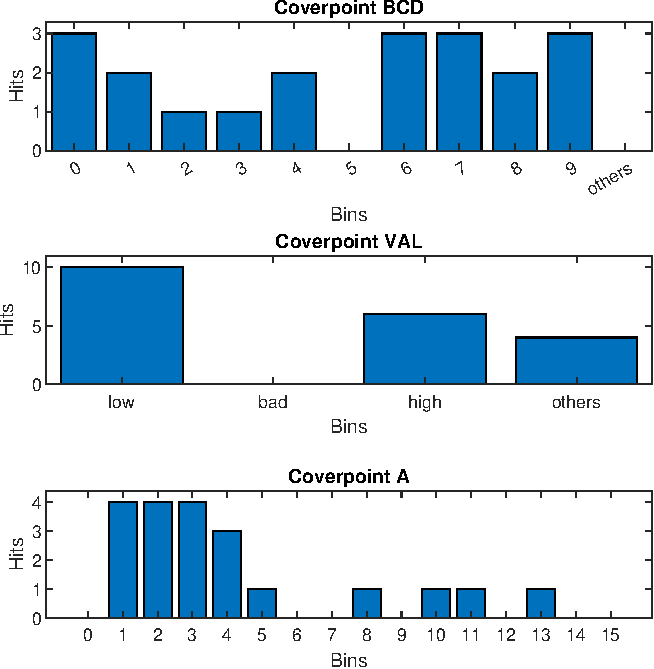
\includegraphics[width=\columnwidth]{coverage.pdf}
	%Figure generated by 'graphs.m'
	\caption{Coverage bins generated by running the code in listing \ref{lst:usingcov}}
\label{fig:coverage}
\end{figure}

\subsection{C integration in Scala}
The \SV DPI is a great addition to the verification workflow, as it allows the designer to easily implement a C model into the \SV testbench.
Similar functionality is available in Scala by leveraging the Java Native Interface (JNI). This is an interface which allows Java / Scala programs to call native code, i.e. code compiled for the specific CPU it is running on. This is typically encountered as .DLL files on Windows or .so files on linux.

When using Chisel and other external libraries, it is recommended to use the Scala Build Tool (sbt) to manage the build. However, doing this makes it more difficult to use the default JNI integration in Scala. This can be alleviated by use of the plugin \texttt{sbt-jni} by Jakob Odersky. 

In listing \ref{lst:jni-scala} is shown an example of a Scala file with a native function.

\begin{listing}[htbp]
\inputminted{scala}{snippets/Myclass.scala}
\caption{Example Scala code showing how to integrate native code in Scala.}
\label{lst:jni-scala}
\end{listing}

The annotation \texttt{@native} informs the Scala compiler that the function should be found in native code. The annotation \texttt{@nativeLoader} is necessary for use with the plugin. The name "native0"\, is the name of the current SBT project, appended with a 0.

Once the above file has been written, the corresponding C header file is generated by running \texttt{sbt javah}. The contents of the generated header file should then be copied into a C code file, where the functions can be implemented. In this case, it may look like the contents of listing \ref{lst:jni-c}.

\begin{listing}[htbp]
\inputminted{C}{snippets/Myclass.c}
\caption{C implementation of the methods declared in Myclass in listing \ref{lst:jni-scala}.}
\label{lst:jni-c}
\end{listing}

Notice that primitives such as \texttt{int} can be autocast from a \texttt{jint}, whereas a string must be obtained used using the function pointers defined in the \texttt{JNIEnv} structure. Once this is done, a CMake makefile is generated by running \texttt{sbt "nativeInit cmake"}, and the C files are compiled using \texttt{sbt nativeCompile}. If all goes well, the code can then be run with \texttt{sbt run}. 

If changes are made to any of the function definitions or Scala file, no other steps are necessary than running \texttt{sbt run} again. This will also invoke the CMake script generation and compilation steps if necessary. If new native methods are added to the Scala file, \texttt{sbt javah} must be run again to generate new C headers.

For more information regarding the plugin setup, see the \href{https://github.com/jodersky/sbt-jni}{plugin page on Github} or the file HowToJni.md in the \href{https://github.com/chisel-uvm/documentation}{documentation repository}.

% *Explain what CRV is
% *Explain what coverage is, how it works
% *Show an example of a coverage histogram.
% TODO Explain the basics of UVM testbenches
% TODO Explain how the SV DPI works
% Explain how the java JNI works
% Collect it all together

\section{From InfinIT}

Digital systems are already an integral part of our life. These systems are built out of microprocessors, application specific integrated circuits (ASICs), and field-programmable gate arrays (FPGAs). Several companies in Denmark are building digital systems. To increase competitivity of those companies, we need tools and methods to increase the productivity in designing and especially testing digital systems. Compared to software development and testing, digital design and testing methods and tools lack several decades of development. Within this project we plan to leverage software development and testing methods for digital design. This project explores the hardware construction language Chisel with Scala and the Universal Verification Method (UVM) with SystemVerilog for design and test of digital systems.



UVM is becoming an industry standard for design verification. On the other hand there is an active development on a new hardware construction language, called Chisel. Chisel is embedded in Scala to write so-called hardware generators. Chisel is also called: software defined hardware. Another feature of the Chisel/Scala combination is to write models of the environment of the hardware design in Scala. As an example take a network interface (e.g., Ethernet) written as a high-level model in Scala connected to a microprocessor written in Chisel. With this example we are able to develop and test network code on the microprocessor, which is our digital design under test.



As a first step we will explore and compare the two approaches: UVM/SystemVerilog and Chisel/Scala. When we generate hardware from Chisel, we generate a Verilog description of the digital circuit. This Verilog description can further be tested within UVM (plain Verilog is valid SystemVerilog). As a next step, we will explore how test, simulation, and verification code written in Scala to develop the Chisel description of the digital circuit can be reused at the UVM level to test the generated Verilog description of the circuit.


Modern software techniques can be applied on testing where plausible. For example, fuzzing is a mature solution for producing random and yet meaningful inputs to trigger program failures. Symbolic execution explores program paths systematically via constraint solving.



We are in contact with the developers of Chisel at the University of California in Berkeley, and especially with Richard Lin, who is developing the new testing framework for Chisel. Richard is interested in this project and the integration with UVM. Therefore, we agreed to have a cooperation meeting during the project at UC Berkeley.



The project fits into the Infinit topic of IoT. The things of IoT are digital systems, often small and application specific systems. Application specific systems are built out of digital systems either with a dedicated ASIC or an FPGA.



This mini-project will be executed in close cooperation with Microchip, WSA, Synopsys, and Syosil. 



The students involved in the research project well then be well educated future engineers for digital system design and verification.



3. Aktiviteter (beskriv) 1. Learning and exploring SystemVerilog/UVM (with Synopsys)
2. Learning and exploring Chisel/Scala
3. Defining two use cases together with Microchip
4. Developing the two use-cases in Chisel and SystemVerilog with a comparison
5. Developing the verification environment including high-level models of the environment in UVM and Chisel/Scala with a comparison
6. Application of the UVM verification of the Chisel generated Verilog code
7. Scala based testing and verification on top of UVM
8. Develop an open course on verification of digital systems for DTU and use in industry




4. MilestonesKnowledge of the tools30/4/2020Definitions of the use cases31/5/2020Use cases developed30/7/2020Verification and high-level models developed31/8/2020Cross verification from Scala to UVM functional, course material finalize31/10/2020

5. Deltagere



DTU, CVR-nr. 30 06 09 46, Martin Schoeberl (project lead) (masca@dtu.dk) and Jan Madsen (jama@dtu.dk)
DTU will develop the use cases and the verification environment with UVM and Chisel/Scala. DTU will transfer knowledge on Chisel to Microchip and WSA.
ITU, CVR-nr. 29 05 77 53, Peter Sestoft (sestoft@itu.dk) and Zhoulai Fu (zhfu@itu.dk)
ITU will apply methods from software testing to digital hardware verification.
Aarhus Universitet, CVR-nr: 31119103, Farshad Moradi (moradi@eng.au.dk)
AU will explore UVM verification of Chisel generated Verilog code.
Microchip Semiconductor Corp. A/S, CVR-nr. 24224694, Thomas Aakjer (Thomas.Aakjer@microchip.com)
Microchip will provide use cases for the research in design and verification where DTU can explore Chisel with Scala.
WS Audiology Denmark A/S, CVR-nr. 40296638, Ketil Julsgaard (ketil.julsgaard@wsa.com)
WSA will provide digital-signal processing use cases for cosimulation of a Chisel description with a high-level description.
Synopsys, CVR-nr. 25600568, Martine Chegaray (Martine.Chegaray@synopsys.com)
Synopsis will provide the tools for UVM for the project and guide the usage.
Syosil Aps, CVR-nr. 29399417, Jacob Sander Andersen (jacob@syosil.com)
Syosil will support the researchers with education in using UVM.


6. Resultater og vision for 

The vision of the project is a highly productive method for designing and (more importantly) verification of digital systems by a combination of the modern hardware construction language Chisel/Scala with the industry standard UVM.
7. Videnspredning

The research work will be documented by publications and presented at relevant conferences (for example DATE), funded by other means, not by this project.

At the end of the project we will present the method at a workshop open for Danish industry in digital system design.

The new development and verification method will be used and taught in courses on digital electronics at DTU.

\end{document}
